%--------------------------------------
%ELECTROTECHNIQUE - SCHEMA DE LIAISON A LA TERRE
%--------------------------------------

%utiliser les environnement \begin{comment} \end{comment} pour mettre en commentaire le préambule une fois la programmation appelée dans le document maître (!ne pas oublier de mettre en commentaire \end{document}!)

\begin{comment}

\documentclass[a4paper, 11pt, twoside, fleqn]{memoir}

\usepackage{AOCDTF}

\marqueurchapitre
\decoupagechapitre{1} %juste pour éviter les erreurs lors de la compilation des sous-programmations (passera en commentaire)

%lien d'édition des figures Tikz sur le site mathcha.io (rajouter le lien d'une modification effectuée sur la figure tikz avec le nom du modificateur car il n'y a qu'un lien par compte)

%lien mathcha Bruno Douchy : https://www.mathcha.io/editor/NXXM3IYwiOphgYY5LKSVg8MmZUL4lDW7U82QN4X

%--------------------------------------
%corps du document
%--------------------------------------

\begin{document} %corps du document
	\openleft %début de chapitre à gauche

\end{comment}


\begin{figure}[H]
\caption{Boucle de courant de défaut $I_{d2}$ du deuxième défaut d'isolement sur L2}
\tikzset{every picture/.style={line width=0.75pt}} %set default line width to 0.75pt        

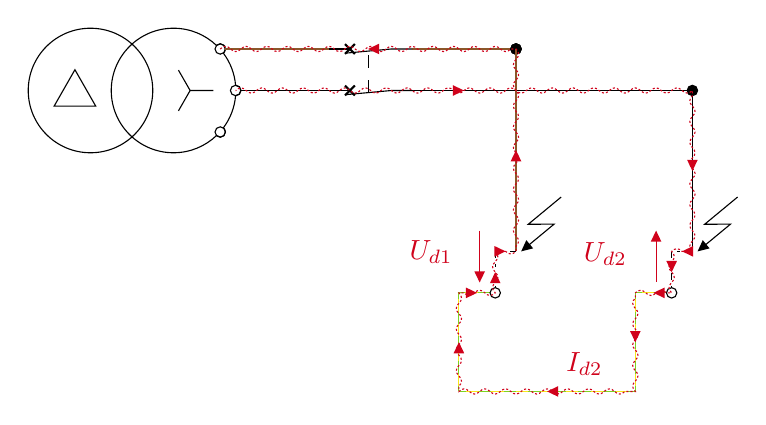
\begin{tikzpicture}[x=0.75pt,y=0.75pt,yscale=-1,xscale=1]
%uncomment if require: \path (0,219); %set diagram left start at 0, and has height of 219

%Straight Lines [id:da4511637283243949] 
\draw  [dash pattern={on 2.25pt off 2.25pt on 1pt off 2.25pt}]  (252.5,112.5) -- (242.5,112.5) -- (242.5,130) ;
%Straight Lines [id:da9527130819146642] 
\draw  [dash pattern={on 2.25pt off 2.25pt on 1pt off 2.25pt}]  (337.5,112.5) -- (327.5,112.5) -- (327.5,130) ;
%Straight Lines [id:da24126717784692808] 
\draw [color={rgb, 255:red, 0; green, 0; blue, 0 }  ,draw opacity=1 ]   (337.5,112.5) -- (337.5,35) ;
%Straight Lines [id:da3468467801372336] 
\draw    (202.5,35) -- (337.5,35) ;
%Straight Lines [id:da5563024891724297] 
\draw [color={rgb, 255:red, 139; green, 87; blue, 42 }  ,draw opacity=1 ]   (202.5,15) -- (252.5,15) ;
%Shape: Path Data [id:dp43837740322366014] 
\draw   (112.5,55) .. controls (112.5,56.38) and (111.38,57.5) .. (110,57.5) .. controls (109.29,57.5) and (108.65,57.2) .. (108.19,56.72) .. controls (102.81,61.85) and (95.52,65) .. (87.5,65) .. controls (70.93,65) and (57.5,51.57) .. (57.5,35) .. controls (57.5,18.43) and (70.93,5) .. (87.5,5) .. controls (95.52,5) and (102.81,8.15) .. (108.19,13.28) .. controls (108.65,12.8) and (109.29,12.5) .. (110,12.5) .. controls (111.38,12.5) and (112.5,13.62) .. (112.5,15) .. controls (112.5,15.82) and (112.11,16.54) .. (111.5,17) .. controls (114.8,21.39) and (116.92,26.71) .. (117.4,32.5) .. controls (117.43,32.5) and (117.47,32.5) .. (117.5,32.5) .. controls (118.88,32.5) and (120,33.62) .. (120,35) .. controls (120,36.38) and (118.88,37.5) .. (117.5,37.5) .. controls (117.47,37.5) and (117.43,37.5) .. (117.4,37.5) .. controls (116.92,43.29) and (114.8,48.61) .. (111.5,53) .. controls (112.11,53.46) and (112.5,54.18) .. (112.5,55) -- cycle ;
%Shape: Circle [id:dp03603482838008654] 
\draw   (17.5,35) .. controls (17.5,18.43) and (30.93,5) .. (47.5,5) .. controls (64.07,5) and (77.5,18.43) .. (77.5,35) .. controls (77.5,51.57) and (64.07,65) .. (47.5,65) .. controls (30.93,65) and (17.5,51.57) .. (17.5,35) -- cycle ;
%Shape: Triangle [id:dp7860018021593028] 
\draw   (40,25) -- (30,42.5) -- (50,42.5) -- cycle ;
%Shape: Star [id:dp36273195667205105] 
\draw   (106.75,35) -- (95.5,35) -- (89.88,44.81) -- (95.5,35) -- (89.88,25.19) -- (95.5,35) -- cycle ;
%Shape: Circle [id:dp581329576165861] 
\draw   (107.5,15) .. controls (107.5,13.62) and (108.62,12.5) .. (110,12.5) .. controls (111.38,12.5) and (112.5,13.62) .. (112.5,15) .. controls (112.5,16.38) and (111.38,17.5) .. (110,17.5) .. controls (108.62,17.5) and (107.5,16.38) .. (107.5,15) -- cycle ;
%Shape: Circle [id:dp008181652335233047] 
\draw   (114.9,35) .. controls (114.9,33.62) and (116.02,32.5) .. (117.4,32.5) .. controls (118.78,32.5) and (119.9,33.62) .. (119.9,35) .. controls (119.9,36.38) and (118.78,37.5) .. (117.4,37.5) .. controls (116.02,37.5) and (114.9,36.38) .. (114.9,35) -- cycle ;
%Shape: Circle [id:dp5428967410526352] 
\draw   (107.5,55) .. controls (107.5,53.62) and (108.62,52.5) .. (110,52.5) .. controls (111.38,52.5) and (112.5,53.62) .. (112.5,55) .. controls (112.5,56.38) and (111.38,57.5) .. (110,57.5) .. controls (108.62,57.5) and (107.5,56.38) .. (107.5,55) -- cycle ;

%Shape: Circle [id:dp3004196596154465] 
\draw  [fill={rgb, 255:red, 0; green, 0; blue, 0 }  ,fill opacity=1 ] (335,35) .. controls (335,33.62) and (336.12,32.5) .. (337.5,32.5) .. controls (338.88,32.5) and (340,33.62) .. (340,35) .. controls (340,36.38) and (338.88,37.5) .. (337.5,37.5) .. controls (336.12,37.5) and (335,36.38) .. (335,35) -- cycle ;
%Shape: Circle [id:dp38478162693673257] 
\draw  [fill={rgb, 255:red, 0; green, 0; blue, 0 }  ,fill opacity=1 ] (250,15) .. controls (250,13.62) and (251.12,12.5) .. (252.5,12.5) .. controls (253.88,12.5) and (255,13.62) .. (255,15) .. controls (255,16.38) and (253.88,17.5) .. (252.5,17.5) .. controls (251.12,17.5) and (250,16.38) .. (250,15) -- cycle ;
%Straight Lines [id:da35747201510733806] 
\draw [color={rgb, 255:red, 139; green, 87; blue, 42 }  ,draw opacity=1 ]   (112.5,15) -- (162.5,15) ;
%Straight Lines [id:da03938247690059582] 
\draw    (120,35) -- (162.5,35) ;
%Shape: Boxed Line [id:dp47312336425022783] 
\draw    (274.27,86.33) -- (258.39,99.47) -- (270.89,99.36) -- (257.31,110.59) ;
\draw [shift={(255,112.5)}, rotate = 320.40999999999997] [fill={rgb, 255:red, 0; green, 0; blue, 0 }  ][line width=0.08]  [draw opacity=0] (5.36,-2.57) -- (0,0) -- (5.36,2.57) -- cycle    ;
%Shape: Boxed Line [id:dp8604246706425941] 
\draw    (359.27,86.33) -- (343.39,99.47) -- (355.89,99.36) -- (342.31,110.59) ;
\draw [shift={(340,112.5)}, rotate = 320.40999999999997] [fill={rgb, 255:red, 0; green, 0; blue, 0 }  ][line width=0.08]  [draw opacity=0] (5.36,-2.57) -- (0,0) -- (5.36,2.57) -- cycle    ;
%Straight Lines [id:da6306782474143875] 
\draw    (170.5,37) -- (192.5,35) -- (202.5,35) ;
%Straight Lines [id:da4629224352649184] 
\draw    (172.5,35) -- (162.5,35) ;
\draw [shift={(172.5,35)}, rotate = 225] [color={rgb, 255:red, 0; green, 0; blue, 0 }  ][line width=0.75]    (-3.35,0) -- (3.35,0)(0,3.35) -- (0,-3.35)   ;
%Straight Lines [id:da5132783320552895] 
\draw    (170.5,17) -- (192.5,15) -- (202.5,15) ;
%Straight Lines [id:da123841191189479] 
\draw  [dash pattern={on 4.5pt off 4.5pt}]  (181.5,36) -- (181.5,16) ;
%Straight Lines [id:da38134434479229706] 
\draw    (172.5,15) -- (162.5,15) ;
\draw [shift={(172.5,15)}, rotate = 225] [color={rgb, 255:red, 0; green, 0; blue, 0 }  ][line width=0.75]    (-3.35,0) -- (3.35,0)(0,3.35) -- (0,-3.35)   ;

%Straight Lines [id:da029862379270012007] 
\draw [color={rgb, 255:red, 139; green, 87; blue, 42 }  ,draw opacity=1 ]   (252.5,112.5) -- (252.5,15) ;
%Shape: Circle [id:dp10157043967465573] 
\draw  [fill={rgb, 255:red, 0; green, 0; blue, 0 }  ,fill opacity=1 ] (250,15) .. controls (250,13.62) and (251.12,12.5) .. (252.5,12.5) .. controls (253.88,12.5) and (255,13.62) .. (255,15) .. controls (255,16.38) and (253.88,17.5) .. (252.5,17.5) .. controls (251.12,17.5) and (250,16.38) .. (250,15) -- cycle ;
%Shape: Circle [id:dp8079725241460669] 
\draw  [fill={rgb, 255:red, 0; green, 0; blue, 0 }  ,fill opacity=1 ] (250,15) .. controls (250,13.62) and (251.12,12.5) .. (252.5,12.5) .. controls (253.88,12.5) and (255,13.62) .. (255,15) .. controls (255,16.38) and (253.88,17.5) .. (252.5,17.5) .. controls (251.12,17.5) and (250,16.38) .. (250,15) -- cycle ;
%Straight Lines [id:da32787816985288987] 
\draw [color={rgb, 255:red, 208; green, 2; blue, 27 }  ,draw opacity=1 ]   (235,102.5) -- (235,124.5) ;
\draw [shift={(235,127.5)}, rotate = 270] [fill={rgb, 255:red, 208; green, 2; blue, 27 }  ,fill opacity=1 ][line width=0.08]  [draw opacity=0] (5.36,-2.57) -- (0,0) -- (5.36,2.57) -- cycle    ;
%Straight Lines [id:da9290035127505091] 
\draw [color={rgb, 255:red, 208; green, 2; blue, 27 }  ,draw opacity=1 ]   (320,105.5) -- (320,127.5) ;
\draw [shift={(320,102.5)}, rotate = 90] [fill={rgb, 255:red, 208; green, 2; blue, 27 }  ,fill opacity=1 ][line width=0.08]  [draw opacity=0] (5.36,-2.57) -- (0,0) -- (5.36,2.57) -- cycle    ;
%Straight Lines [id:da4236883272393758] 
\draw [color={rgb, 255:red, 248; green, 231; blue, 28 }  ,draw opacity=1 ]   (325,132.5) -- (310,132.5) -- (310,180) -- (225,180) ;
%Straight Lines [id:da1955939853197214] 
\draw [color={rgb, 255:red, 126; green, 211; blue, 33 }  ,draw opacity=1 ] [dash pattern={on 4.5pt off 4.5pt}]  (325,132.5) -- (310,132.5) -- (310,180) -- (225,180) ;
%Straight Lines [id:da8052192234703028] 
\draw [color={rgb, 255:red, 248; green, 231; blue, 28 }  ,draw opacity=1 ]   (240,132.5) -- (225,132.5) -- (225,180) ;
%Straight Lines [id:da6976347779102222] 
\draw [color={rgb, 255:red, 139; green, 87; blue, 42 }  ,draw opacity=1 ]   (252.5,110) -- (252.5,15) ;
%Straight Lines [id:da2970008681971681] 
\draw [color={rgb, 255:red, 126; green, 211; blue, 33 }  ,draw opacity=1 ] [dash pattern={on 4.5pt off 4.5pt}]  (240,132.5) -- (225,132.5) -- (225,180) ;
%Straight Lines [id:da7142618830255841] 
\draw [color={rgb, 255:red, 0; green, 0; blue, 0 }  ,draw opacity=1 ]   (337.5,110) -- (337.5,32.5) ;
%Shape: Circle [id:dp970057374964288] 
\draw  [fill={rgb, 255:red, 255; green, 255; blue, 255 }  ,fill opacity=1 ] (240,132.5) .. controls (240,131.12) and (241.12,130) .. (242.5,130) .. controls (243.88,130) and (245,131.12) .. (245,132.5) .. controls (245,133.88) and (243.88,135) .. (242.5,135) .. controls (241.12,135) and (240,133.88) .. (240,132.5) -- cycle ;
%Shape: Circle [id:dp5285112483449262] 
\draw  [fill={rgb, 255:red, 255; green, 255; blue, 255 }  ,fill opacity=1 ] (325,132.5) .. controls (325,131.12) and (326.12,130) .. (327.5,130) .. controls (328.88,130) and (330,131.12) .. (330,132.5) .. controls (330,133.88) and (328.88,135) .. (327.5,135) .. controls (326.12,135) and (325,133.88) .. (325,132.5) -- cycle ;
%Straight Lines [id:da2635484251048684] 
\draw [color={rgb, 255:red, 208; green, 2; blue, 27 }  ,draw opacity=1 ] [dash pattern={on 0.75pt off 0.75pt}]  (110,15) .. controls (111.67,13.33) and (113.33,13.33) .. (115,15) .. controls (116.67,16.67) and (118.33,16.67) .. (120,15) .. controls (121.67,13.33) and (123.33,13.33) .. (125,15) .. controls (126.67,16.67) and (128.33,16.67) .. (130,15) .. controls (131.67,13.33) and (133.33,13.33) .. (135,15) .. controls (136.67,16.67) and (138.33,16.67) .. (140,15) .. controls (141.67,13.33) and (143.33,13.33) .. (145,15) .. controls (146.67,16.67) and (148.33,16.67) .. (150,15) .. controls (151.67,13.33) and (153.33,13.33) .. (155,15) .. controls (156.67,16.67) and (158.33,16.67) .. (160,15) .. controls (161.67,13.33) and (163.33,13.33) .. (165,15) .. controls (166.67,16.67) and (168.33,16.67) .. (170,15) .. controls (171.67,13.33) and (173.33,13.33) .. (175,15) .. controls (176.67,16.67) and (178.33,16.67) .. (180,15) .. controls (181.67,13.33) and (183.33,13.33) .. (185,15) .. controls (186.67,16.67) and (188.33,16.67) .. (190,15) .. controls (191.67,13.33) and (193.33,13.33) .. (195,15) .. controls (196.67,16.67) and (198.33,16.67) .. (200,15) .. controls (201.67,13.33) and (203.33,13.33) .. (205,15) .. controls (206.67,16.67) and (208.33,16.67) .. (210,15) .. controls (211.67,13.33) and (213.33,13.33) .. (215,15) .. controls (216.67,16.67) and (218.33,16.67) .. (220,15) .. controls (221.67,13.33) and (223.33,13.33) .. (225,15) .. controls (226.67,16.67) and (228.33,16.67) .. (230,15) .. controls (231.67,13.33) and (233.33,13.33) .. (235,15) .. controls (236.67,16.67) and (238.33,16.67) .. (240,15) .. controls (241.67,13.33) and (243.33,13.33) .. (245,15) .. controls (246.67,16.67) and (248.33,16.67) .. (250,15) -- (252.5,15) -- (252.5,15) .. controls (254.17,16.67) and (254.17,18.33) .. (252.5,20) .. controls (250.83,21.67) and (250.83,23.33) .. (252.5,25) .. controls (254.17,26.67) and (254.17,28.33) .. (252.5,30) .. controls (250.83,31.67) and (250.83,33.33) .. (252.5,35) .. controls (254.17,36.67) and (254.17,38.33) .. (252.5,40) .. controls (250.83,41.67) and (250.83,43.33) .. (252.5,45) .. controls (254.17,46.67) and (254.17,48.33) .. (252.5,50) .. controls (250.83,51.67) and (250.83,53.33) .. (252.5,55) .. controls (254.17,56.67) and (254.17,58.33) .. (252.5,60) .. controls (250.83,61.67) and (250.83,63.33) .. (252.5,65) .. controls (254.17,66.67) and (254.17,68.33) .. (252.5,70) .. controls (250.83,71.67) and (250.83,73.33) .. (252.5,75) .. controls (254.17,76.67) and (254.17,78.33) .. (252.5,80) .. controls (250.83,81.67) and (250.83,83.33) .. (252.5,85) .. controls (254.17,86.67) and (254.17,88.33) .. (252.5,90) .. controls (250.83,91.67) and (250.83,93.33) .. (252.5,95) .. controls (254.17,96.67) and (254.17,98.33) .. (252.5,100) .. controls (250.83,101.67) and (250.83,103.33) .. (252.5,105) .. controls (254.17,106.67) and (254.17,108.33) .. (252.5,110) -- (252.5,112.5) -- (252.5,112.5) .. controls (250.83,114.17) and (249.17,114.17) .. (247.5,112.5) -- (242.5,112.5) -- (242.5,112.5) .. controls (244.17,114.17) and (244.17,115.83) .. (242.5,117.5) .. controls (240.83,119.17) and (240.83,120.83) .. (242.5,122.5) .. controls (244.17,124.17) and (244.17,125.83) .. (242.5,127.5) .. controls (240.83,129.17) and (240.83,130.83) .. (242.5,132.5) -- (242.5,132.5) .. controls (240.83,134.17) and (239.17,134.17) .. (237.5,132.5) .. controls (235.83,130.83) and (234.17,130.83) .. (232.5,132.5) .. controls (230.83,134.17) and (229.17,134.17) .. (227.5,132.5) -- (225,132.5) -- (225,132.5) .. controls (226.67,134.17) and (226.67,135.83) .. (225,137.5) .. controls (223.33,139.17) and (223.33,140.83) .. (225,142.5) .. controls (226.67,144.17) and (226.67,145.83) .. (225,147.5) .. controls (223.33,149.17) and (223.33,150.83) .. (225,152.5) .. controls (226.67,154.17) and (226.67,155.83) .. (225,157.5) .. controls (223.33,159.17) and (223.33,160.83) .. (225,162.5) .. controls (226.67,164.17) and (226.67,165.83) .. (225,167.5) .. controls (223.33,169.17) and (223.33,170.83) .. (225,172.5) .. controls (226.67,174.17) and (226.67,175.83) .. (225,177.5) -- (225,180) -- (225,180) .. controls (226.67,178.33) and (228.33,178.33) .. (230,180) .. controls (231.67,181.67) and (233.33,181.67) .. (235,180) .. controls (236.67,178.33) and (238.33,178.33) .. (240,180) .. controls (241.67,181.67) and (243.33,181.67) .. (245,180) .. controls (246.67,178.33) and (248.33,178.33) .. (250,180) .. controls (251.67,181.67) and (253.33,181.67) .. (255,180) .. controls (256.67,178.33) and (258.33,178.33) .. (260,180) .. controls (261.67,181.67) and (263.33,181.67) .. (265,180) .. controls (266.67,178.33) and (268.33,178.33) .. (270,180) .. controls (271.67,181.67) and (273.33,181.67) .. (275,180) .. controls (276.67,178.33) and (278.33,178.33) .. (280,180) .. controls (281.67,181.67) and (283.33,181.67) .. (285,180) .. controls (286.67,178.33) and (288.33,178.33) .. (290,180) .. controls (291.67,181.67) and (293.33,181.67) .. (295,180) .. controls (296.67,178.33) and (298.33,178.33) .. (300,180) .. controls (301.67,181.67) and (303.33,181.67) .. (305,180) -- (310,180) -- (310,180) .. controls (308.33,178.33) and (308.33,176.67) .. (310,175) .. controls (311.67,173.33) and (311.67,171.67) .. (310,170) .. controls (308.33,168.33) and (308.33,166.67) .. (310,165) .. controls (311.67,163.33) and (311.67,161.67) .. (310,160) .. controls (308.33,158.33) and (308.33,156.67) .. (310,155) .. controls (311.67,153.33) and (311.67,151.67) .. (310,150) .. controls (308.33,148.33) and (308.33,146.67) .. (310,145) .. controls (311.67,143.33) and (311.67,141.67) .. (310,140) .. controls (308.33,138.33) and (308.33,136.67) .. (310,135) -- (310,132.5) -- (310,132.5) .. controls (311.67,130.83) and (313.33,130.83) .. (315,132.5) .. controls (316.67,134.17) and (318.33,134.17) .. (320,132.5) .. controls (321.67,130.83) and (323.33,130.83) .. (325,132.5) -- (327.5,132.5) -- (327.5,132.5) .. controls (325.83,130.83) and (325.83,129.17) .. (327.5,127.5) .. controls (329.17,125.83) and (329.17,124.17) .. (327.5,122.5) .. controls (325.83,120.83) and (325.83,119.17) .. (327.5,117.5) .. controls (329.17,115.83) and (329.17,114.17) .. (327.5,112.5) -- (327.5,112.5) .. controls (329.17,110.83) and (330.83,110.83) .. (332.5,112.5) -- (337.5,112.5) -- (337.5,112.5) .. controls (335.83,110.83) and (335.83,109.17) .. (337.5,107.5) .. controls (339.17,105.83) and (339.17,104.17) .. (337.5,102.5) .. controls (335.83,100.83) and (335.83,99.17) .. (337.5,97.5) .. controls (339.17,95.83) and (339.17,94.17) .. (337.5,92.5) .. controls (335.83,90.83) and (335.83,89.17) .. (337.5,87.5) .. controls (339.17,85.83) and (339.17,84.17) .. (337.5,82.5) .. controls (335.83,80.83) and (335.83,79.17) .. (337.5,77.5) .. controls (339.17,75.83) and (339.17,74.17) .. (337.5,72.5) .. controls (335.83,70.83) and (335.83,69.17) .. (337.5,67.5) .. controls (339.17,65.83) and (339.17,64.17) .. (337.5,62.5) .. controls (335.83,60.83) and (335.83,59.17) .. (337.5,57.5) .. controls (339.17,55.83) and (339.17,54.17) .. (337.5,52.5) .. controls (335.83,50.83) and (335.83,49.17) .. (337.5,47.5) .. controls (339.17,45.83) and (339.17,44.17) .. (337.5,42.5) .. controls (335.83,40.83) and (335.83,39.17) .. (337.5,37.5) -- (337.5,35) -- (337.5,35) .. controls (335.83,36.67) and (334.17,36.67) .. (332.5,35) .. controls (330.83,33.33) and (329.17,33.33) .. (327.5,35) .. controls (325.83,36.67) and (324.17,36.67) .. (322.5,35) .. controls (320.83,33.33) and (319.17,33.33) .. (317.5,35) .. controls (315.83,36.67) and (314.17,36.67) .. (312.5,35) .. controls (310.83,33.33) and (309.17,33.33) .. (307.5,35) .. controls (305.83,36.67) and (304.17,36.67) .. (302.5,35) .. controls (300.83,33.33) and (299.17,33.33) .. (297.5,35) .. controls (295.83,36.67) and (294.17,36.67) .. (292.5,35) .. controls (290.83,33.33) and (289.17,33.33) .. (287.5,35) .. controls (285.83,36.67) and (284.17,36.67) .. (282.5,35) .. controls (280.83,33.33) and (279.17,33.33) .. (277.5,35) .. controls (275.83,36.67) and (274.17,36.67) .. (272.5,35) .. controls (270.83,33.33) and (269.17,33.33) .. (267.5,35) .. controls (265.83,36.67) and (264.17,36.67) .. (262.5,35) .. controls (260.83,33.33) and (259.17,33.33) .. (257.5,35) .. controls (255.83,36.67) and (254.17,36.67) .. (252.5,35) .. controls (250.83,33.33) and (249.17,33.33) .. (247.5,35) .. controls (245.83,36.67) and (244.17,36.67) .. (242.5,35) .. controls (240.83,33.33) and (239.17,33.33) .. (237.5,35) .. controls (235.83,36.67) and (234.17,36.67) .. (232.5,35) .. controls (230.83,33.33) and (229.17,33.33) .. (227.5,35) .. controls (225.83,36.67) and (224.17,36.67) .. (222.5,35) .. controls (220.83,33.33) and (219.17,33.33) .. (217.5,35) .. controls (215.83,36.67) and (214.17,36.67) .. (212.5,35) .. controls (210.83,33.33) and (209.17,33.33) .. (207.5,35) .. controls (205.83,36.67) and (204.17,36.67) .. (202.5,35) .. controls (200.83,33.33) and (199.17,33.33) .. (197.5,35) .. controls (195.83,36.67) and (194.17,36.67) .. (192.5,35) .. controls (190.83,33.33) and (189.17,33.33) .. (187.5,35) .. controls (185.83,36.67) and (184.17,36.67) .. (182.5,35) .. controls (180.83,33.33) and (179.17,33.33) .. (177.5,35) .. controls (175.83,36.67) and (174.17,36.67) .. (172.5,35) .. controls (170.83,33.33) and (169.17,33.33) .. (167.5,35) .. controls (165.83,36.67) and (164.17,36.67) .. (162.5,35) .. controls (160.83,33.33) and (159.17,33.33) .. (157.5,35) .. controls (155.83,36.67) and (154.17,36.67) .. (152.5,35) .. controls (150.83,33.33) and (149.17,33.33) .. (147.5,35) .. controls (145.83,36.67) and (144.17,36.67) .. (142.5,35) .. controls (140.83,33.33) and (139.17,33.33) .. (137.5,35) .. controls (135.83,36.67) and (134.17,36.67) .. (132.5,35) .. controls (130.83,33.33) and (129.17,33.33) .. (127.5,35) .. controls (125.83,36.67) and (124.17,36.67) .. (122.5,35) .. controls (120.83,33.33) and (119.17,33.33) .. (117.5,35) -- (117.4,35) -- (117.4,35) ;
\draw [shift={(181.25,15)}, rotate = 0] [fill={rgb, 255:red, 208; green, 2; blue, 27 }  ,fill opacity=1 ][line width=0.08]  [draw opacity=0] (5.36,-2.57) -- (0,0) -- (5.36,2.57) -- cycle    ;
\draw [shift={(252.5,63.75)}, rotate = 90] [fill={rgb, 255:red, 208; green, 2; blue, 27 }  ,fill opacity=1 ][line width=0.08]  [draw opacity=0] (5.36,-2.57) -- (0,0) -- (5.36,2.57) -- cycle    ;
\draw [shift={(247.5,112.5)}, rotate = 180] [fill={rgb, 255:red, 208; green, 2; blue, 27 }  ,fill opacity=1 ][line width=0.08]  [draw opacity=0] (5.36,-2.57) -- (0,0) -- (5.36,2.57) -- cycle    ;
\draw [shift={(242.5,122.5)}, rotate = 90] [fill={rgb, 255:red, 208; green, 2; blue, 27 }  ,fill opacity=1 ][line width=0.08]  [draw opacity=0] (5.36,-2.57) -- (0,0) -- (5.36,2.57) -- cycle    ;
\draw [shift={(233.75,132.5)}, rotate = 180] [fill={rgb, 255:red, 208; green, 2; blue, 27 }  ,fill opacity=1 ][line width=0.08]  [draw opacity=0] (5.36,-2.57) -- (0,0) -- (5.36,2.57) -- cycle    ;
\draw [shift={(225,156.25)}, rotate = 90] [fill={rgb, 255:red, 208; green, 2; blue, 27 }  ,fill opacity=1 ][line width=0.08]  [draw opacity=0] (5.36,-2.57) -- (0,0) -- (5.36,2.57) -- cycle    ;
\draw [shift={(267.5,180)}, rotate = 0] [fill={rgb, 255:red, 208; green, 2; blue, 27 }  ,fill opacity=1 ][line width=0.08]  [draw opacity=0] (5.36,-2.57) -- (0,0) -- (5.36,2.57) -- cycle    ;
\draw [shift={(310,156.25)}, rotate = 270] [fill={rgb, 255:red, 208; green, 2; blue, 27 }  ,fill opacity=1 ][line width=0.08]  [draw opacity=0] (5.36,-2.57) -- (0,0) -- (5.36,2.57) -- cycle    ;
\draw [shift={(318.75,132.5)}, rotate = 0] [fill={rgb, 255:red, 208; green, 2; blue, 27 }  ,fill opacity=1 ][line width=0.08]  [draw opacity=0] (5.36,-2.57) -- (0,0) -- (5.36,2.57) -- cycle    ;
\draw [shift={(327.5,122.5)}, rotate = 270] [fill={rgb, 255:red, 208; green, 2; blue, 27 }  ,fill opacity=1 ][line width=0.08]  [draw opacity=0] (5.36,-2.57) -- (0,0) -- (5.36,2.57) -- cycle    ;
\draw [shift={(332.5,112.5)}, rotate = 0] [fill={rgb, 255:red, 208; green, 2; blue, 27 }  ,fill opacity=1 ][line width=0.08]  [draw opacity=0] (5.36,-2.57) -- (0,0) -- (5.36,2.57) -- cycle    ;
\draw [shift={(337.5,73.75)}, rotate = 270] [fill={rgb, 255:red, 208; green, 2; blue, 27 }  ,fill opacity=1 ][line width=0.08]  [draw opacity=0] (5.36,-2.57) -- (0,0) -- (5.36,2.57) -- cycle    ;
\draw [shift={(227.45,35)}, rotate = 180] [fill={rgb, 255:red, 208; green, 2; blue, 27 }  ,fill opacity=1 ][line width=0.08]  [draw opacity=0] (5.36,-2.57) -- (0,0) -- (5.36,2.57) -- cycle    ;


% Text Node
\draw (275.5,160) node [anchor=north west][inner sep=0.75pt]  [color={rgb, 255:red, 208; green, 2; blue, 27 }  ,opacity=1 ] [align=left] {$I_{d2}$};
% Text Node
\draw (200,106) node [anchor=north west][inner sep=0.75pt]  [color={rgb, 255:red, 208; green, 2; blue, 27 }  ,opacity=1 ] [align=left] {$U_{d1}$};
% Text Node
\draw (284,107) node [anchor=north west][inner sep=0.75pt]  [color={rgb, 255:red, 208; green, 2; blue, 27 }  ,opacity=1 ] [align=left] {$U_{d2}$};


\end{tikzpicture}


\end{figure}

%\end{document}
